\documentclass{standalone}
\usepackage{tikz}
\usepackage{ctex,siunitx,ninecolors}
\setCJKmainfont{Noto Serif CJK SC}
\usepackage{tkz-euclide}
\usepackage{amsmath}
\usetikzlibrary{patterns, calc}
\usetikzlibrary {decorations.pathmorphing, decorations.pathreplacing, decorations.shapes}
\begin{document}
\small
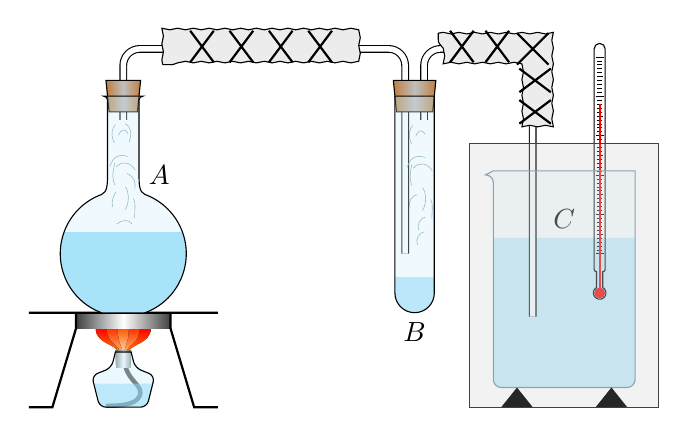
\begin{tikzpicture}[>=latex,scale=1.0]
  % \useasboundingbox(-1.4,-1.4)rectangle(1.4,1.4);
  \fill[top color=red,bottom color=orange](-0.35,1)..controls(-0.35,0.8)and(-0.075,0.8)..(-0.075,0.7)--(0.075,0.7)..controls(0.075,0.8)and(0.35,0.8)..(0.35,1);
  \fill[top color=red!60!orange,bottom color=orange!60](-0.21,1)..controls(-0.21,0.8)and(-0.045,0.8)..(-0.045,0.7)--(0.045,0.7)..controls(0.045,0.8)and(0.21,0.8)..(0.21,1);
  \fill[top color=red!30!orange,bottom color=orange!30](-0.07,1)..controls(-0.07,0.8)and(-0.015,0.8)..(-0.015,0.7)--(0.015,0.7)..controls(0.015,0.8)and(0.07,0.8)..(0.07,1);
  \draw[ultra thick,darkgray]( 0.000,0.700)..controls( 0.000,0.300)and( 0.296,0.300)..( 0.197,0.123)..controls( 0.136,0.032)and(-0.021,0.017)..(-0.222,0.018);
  \fill[rounded corners=0.8mm,cyan!60,opacity=0.5](-0.375,0.3)--(-0.3,0)--(0.3,0)--(0.375,0.3);
  \fill[left color=gray,right color=gray,middle color=white](-0.1010,0.72)--(-0.09,0.5)--(0.09,0.5)--(0.1010,0.72);
  \draw[rounded corners=0.8mm,fill=cyan!20,fill opacity=0.4](-0.1,0.7)--(-0.15,0.5)--(-0.4,0.4)--(-0.3,0)--(0.3,0)--(0.4,0.4)--(0.15,0.5)[sharp corners]--(0.1,0.7)--cycle;

  \fill[left color=darkgray,right color=darkgray,middle color=white](-0.6,1.2)rectangle(0.6,1.0);
  \draw[thick](-1.2,1.2)--(1.2,1.2)(-0.6,1.2)--(-0.6,1.0)--(-0.9,0)--(-1.2,0)(0.6,1.2)--(0.6,1.0)--(0.9,0)--(1.2,0);

  \begin{scope}[yshift=1.95cm]
    \fill[cyan!40!white](160:0.8)arc(160:250:0.8)--(290:0.8)arc(290:380:0.8);
    \fill[cyan!30!white](3.45,-0.3)--(3.45,-0.5)arc(-180:0:0.25)--(3.95,-0.3);
    \fill[cyan!70!white,opacity=0.3](4.7,0.2)--(4.7,-1.6)arc(-180:-90:0.1)--(6.4,-1.7)arc(-90:0:0.1)--(6.5,0.2);
    \node at (5.6,0.2)[above]{$C$};
    \foreach \y in {0,0.5,...,2}
    {
      \draw[ultra thin](6.0,\y)--++(0.1,0);
      \draw[ultra thin](6.01,\y+0.25)--++(0.08,0);
      \foreach \z in {1,2,3,4,6,7,8,9}
      {
        \draw[ultra thin](6.02,\y+0.05*\z)--++(0.06,0);
      }
    }
    \draw[ultra thin](6.0,2.5)--++(0.1,0);
    \draw(5.98,-0.2)--(5.98,2.6)arc(180:0:0.07)--(6.12,-0.2)arc(0:-90:0.03)--++(0,-0.2)arc(420:120:0.08)--++(0,0.2)arc(-90:-180:0.03);
    \fill[red](6.05,-0.5)circle(0.07);
    \draw[thick,red](6.05,-0.5)--++(0,2.4);
    \draw[double,double distance=2pt,rounded corners=6pt](0,1.7)--(0,2.6)--(3.58,2.6)--(3.58,0)(3.82,1.7)--(3.82,2.6)--(5.2,2.6)--(5.2,-0.8);
    \draw[decorate,decoration={snake,segment length =2mm,amplitude=0.1mm},fill=lightgray!30](0.5,2.4)rectangle(3,2.8);
    \foreach \x in {1.0,1.5,...,2.5}
    {
      \draw[thick](\x,2.63)--++(0.15,0.2)(\x,2.63)--++(-0.15,-0.2)(\x,2.63)--++(-0.15,0.2)(\x,2.63)--++(0.15,-0.2);
    }
    \draw[decorate,decoration={snake,segment length =2mm,amplitude=0.1mm},fill=lightgray!30](4.0,2.8)--(5.4,2.8)--(5.4,1.6)--(5.0,1.6)--(5.0,2.4)--(4.0,2.4)--cycle;
    \draw[thick](5.0,2.4)--(5.4,2.8)(5.0,2.8)--(5.4,2.4);
    \foreach \x in {4.3,4.75}
    {
      \draw[thick](\x,2.63)--++(0.15,0.2)(\x,2.63)--++(-0.15,-0.2)(\x,2.63)--++(-0.15,0.2)(\x,2.63)--++(0.15,-0.2);
    }
    \foreach \x in {1.8,2.2}
    {
      \draw[thick](5.23,\x)--++(0.2,0.15)(5.23,\x)--++(-0.2,-0.15)(5.23,\x)--++(0.2,-0.15)(5.23,\x)--++(-0.2,0.15);
    }
  \draw[left color=brown,right color=brown,middle color=lightgray](3.47,1.8)--(3.43,2.2)--(3.97,2.2)--(3.93,1.8)--cycle;
  \node at (3.7,-0.75) [below]{$B$};
  \draw[left color=brown,right color=brown,middle color=lightgray](-0.18,1.8)--(-0.22,2.2)--(0.22,2.2)--(0.18,1.8)--cycle;

  \draw[very thin,cyan!30!gray]
  (-0.113,1.405)..controls(-0.169,1.513)and(-0.136,1.608)..(-0.098,1.639)
(-0.059,1.502)..controls(-0.029,1.589)and( 0.030,1.589)..( 0.060,1.524)
( 0.024,1.649)..controls( 0.106,1.604)and( 0.109,1.536)..( 0.076,1.416)
(-0.171,1.105)..controls(-0.128,1.237)and(-0.055,1.267)..( 0.060,1.234)
(-0.090,1.098)..controls(-0.028,1.177)and( 0.089,1.171)..( 0.150,1.060)
(-0.109,0.874)..controls(-0.154,0.986)and(-0.119,1.087)..(-0.109,1.149)
( 0.049,1.018)..controls( 0.150,0.967)and( 0.157,0.909)..( 0.146,0.821)
( 0.025,0.560)..controls( 0.080,0.648)and( 0.074,0.780)..( 0.027,0.848)
(-0.135,0.595)..controls(-0.162,0.666)and(-0.109,0.754)..(-0.097,0.783)
( 0.143,0.453)..controls( 0.150,0.586)and( 0.157,0.657)..( 0.129,0.699)
(-0.079,0.377)..controls(-0.021,0.433)and( 0.076,0.437)..( 0.111,0.375)
( 3.735,0.112)..controls( 3.707,0.183)and( 3.760,0.271)..( 3.824,0.276)
( 3.751,0.300)..controls( 3.724,0.371)and( 3.777,0.459)..( 3.840,0.464)
( 3.918,0.441)..controls( 3.925,0.575)and( 3.932,0.645)..( 3.904,0.687)
( 3.800,0.548)..controls( 3.855,0.636)and( 3.850,0.768)..( 3.802,0.837)
( 3.641,0.584)..controls( 3.613,0.654)and( 3.666,0.742)..( 3.730,0.747)
( 3.666,0.863)..controls( 3.622,0.975)and( 3.656,1.076)..( 3.666,1.138)
( 3.686,1.086)..controls( 3.748,1.165)and( 3.864,1.160)..( 3.925,1.049)
( 3.604,1.093)..controls( 3.647,1.226)and( 3.720,1.255)..( 3.835,1.222)
( 3.662,1.394)..controls( 3.607,1.502)and( 3.640,1.597)..( 3.678,1.628)
( 3.716,1.491)..controls( 3.746,1.578)and( 3.805,1.578)..( 3.835,1.513);

  \draw[fill=cyan!20,fill opacity=0.3](3.45,2)--(3.45,-0.5)arc(-180:0:0.25)--(3.95,2)--cycle;
  \draw[fill=cyan!20,fill opacity=0.3](0,2.0)--(-0.25,2.0)arc(90:0:0.05)--(-0.2,1)..controls(-0.2,0.9)and(-0.2,0.7785)..(110:0.8)arc(110:250:0.8)--(290:0.8)arc(290:430:0.8)..controls(0.2,0.7785)and(0.2,0.9)..(0.2,1)node[text=black,opacity=1,right]{$A$}--(0.2,1.95)arc(180:90:0.05)--cycle;
  \draw[cyan!30!gray,fill=cyan!20,fill opacity=0.2](4.6,1.0)arc(90:0:0.1)--(4.7,-1.6)arc(-180:-90:0.1)--(6.4,-1.7)arc(-90:0:0.1)--(6.5,1.05)--(4.7,1.05)--cycle;
  \fill(5.0,-1.7)--++(-0.2,-0.25)--++(0.4,0)(6.2,-1.7)--++(-0.2,-0.25)--++(0.4,0);
  \draw[darkgray,fill=lightgray,fill opacity=0.2](4.4,-1.95)rectangle(6.8,1.4);
  \end{scope}
\end{tikzpicture}
\end{document}